\section{Pianificazione}
I diagrammi delle attività presenti in questa sezione sono stati rappresentati 
tramite l'uso di diagrammi di Gantt\G.

\subsection{Analisi dei Requisiti}
\textbf{Periodo:} 04/03/2016 - 31/03/2016\\
Questa fase prevedere la scelta e l'implementazione degli strumenti necessari 
per definire il \textit{repository}\G\ utilizzato dal \textit{team}, le 
norme di base per sviluppare una documentazione quanto più possibile omogenea e 
coerente, una pianificazione che guida lo sviluppo del progetto. Termina con 
la scadenza di consegna dell'offerta, cioè con la consegna della 
\textit{Revisione dei Requisiti}.\\\\
I ruoli attivi in questa fase sono:

\begin{itemize}
	\item Responsabile;
	\item Amministratore;
	\item Analista;
	\item Verificatore.
\end{itemize}
Le attività da svolgersi in questa fase sono:
\begin{itemize}
	\item \textbf{Ricerca ed implementazione degli strumenti}: 
	l'\textit{Amministratore di Progetto} ha il compito di scegliere, 
	implementare e configurare gli strumenti necessari al lavoro del team. Deve 
	apprendere il funzionamento e fare formazione ai rimanenti membri del 
	\textit{team} di sviluppo;
	\item \textbf{Norme di Progetto}: attività svolta 
	dall'\textit{Amministratore di 
	Progetto}. Concordati con il \textit{team} gli strumenti da utilizzare, 
	si procede 	alla stesura di un serie di norme, che dovranno essere 
	rispettate dai membri del team per tutta la durata del progetto. Le norme 
	sono interne al \textit{team} e non legate al capitolato SiVoDiM;
	\item \textbf{Studio di fattibilità}: è compito degli \textit{Analisti} 
	valutare ogni capitolato e redigere uno Studio di fattibilità, dal quale si 
	delinea chiaramente quale capitolato è stato scelto e la motivazione che ha 
	guidato a tale scelta.
	\item \textbf{Piano di Progetto}: qui vengono pianificate attività, 
	risorse e costi per la gestione del \textit{team}. Esse sono riportate in modo 
	strutturato nel \textit{Piano di Progetto v1.0.0};
	\item \textbf{Analisi dei Requisiti}: gli \textit{Analisti} hanno 
	l'incarico di ricercare i requisiti e di redigere il documento 
	\textit{Analisi dei Requisiti v1.0.0}, con Diagrammi dei Casi D'Uso (UC\G). 
	Questa attività è poco legata	al Proponente, data la natura vaga del 
	Capitolato fornito dall'azienda MIVOQ s.r.l.;
	\item \textbf{Piano di Qualifica}: descrizione delle strategie di verifica e 
	validazione adottate. Documentate nel \textit{Piano di Progetto v1.0.0};
	\item \textbf{Glossario}: attività parallela alla stesura di tutti i 
	documenti sopracitati. Il \textit{Glossario v1.0.0} deve essere aggiornato in 
	modo incrementale fino al completamento della documentazione;
	\item \textbf{Verbale incontri}: per analizzare i requisiti presentati nel 
	Capitolato vengono organizzati degli incontri, in seguito documentati con dei 
	verbali.
\end{itemize}

\subsubsection{Diagramma WBS}
\begin{figure}[H]
	\centering
	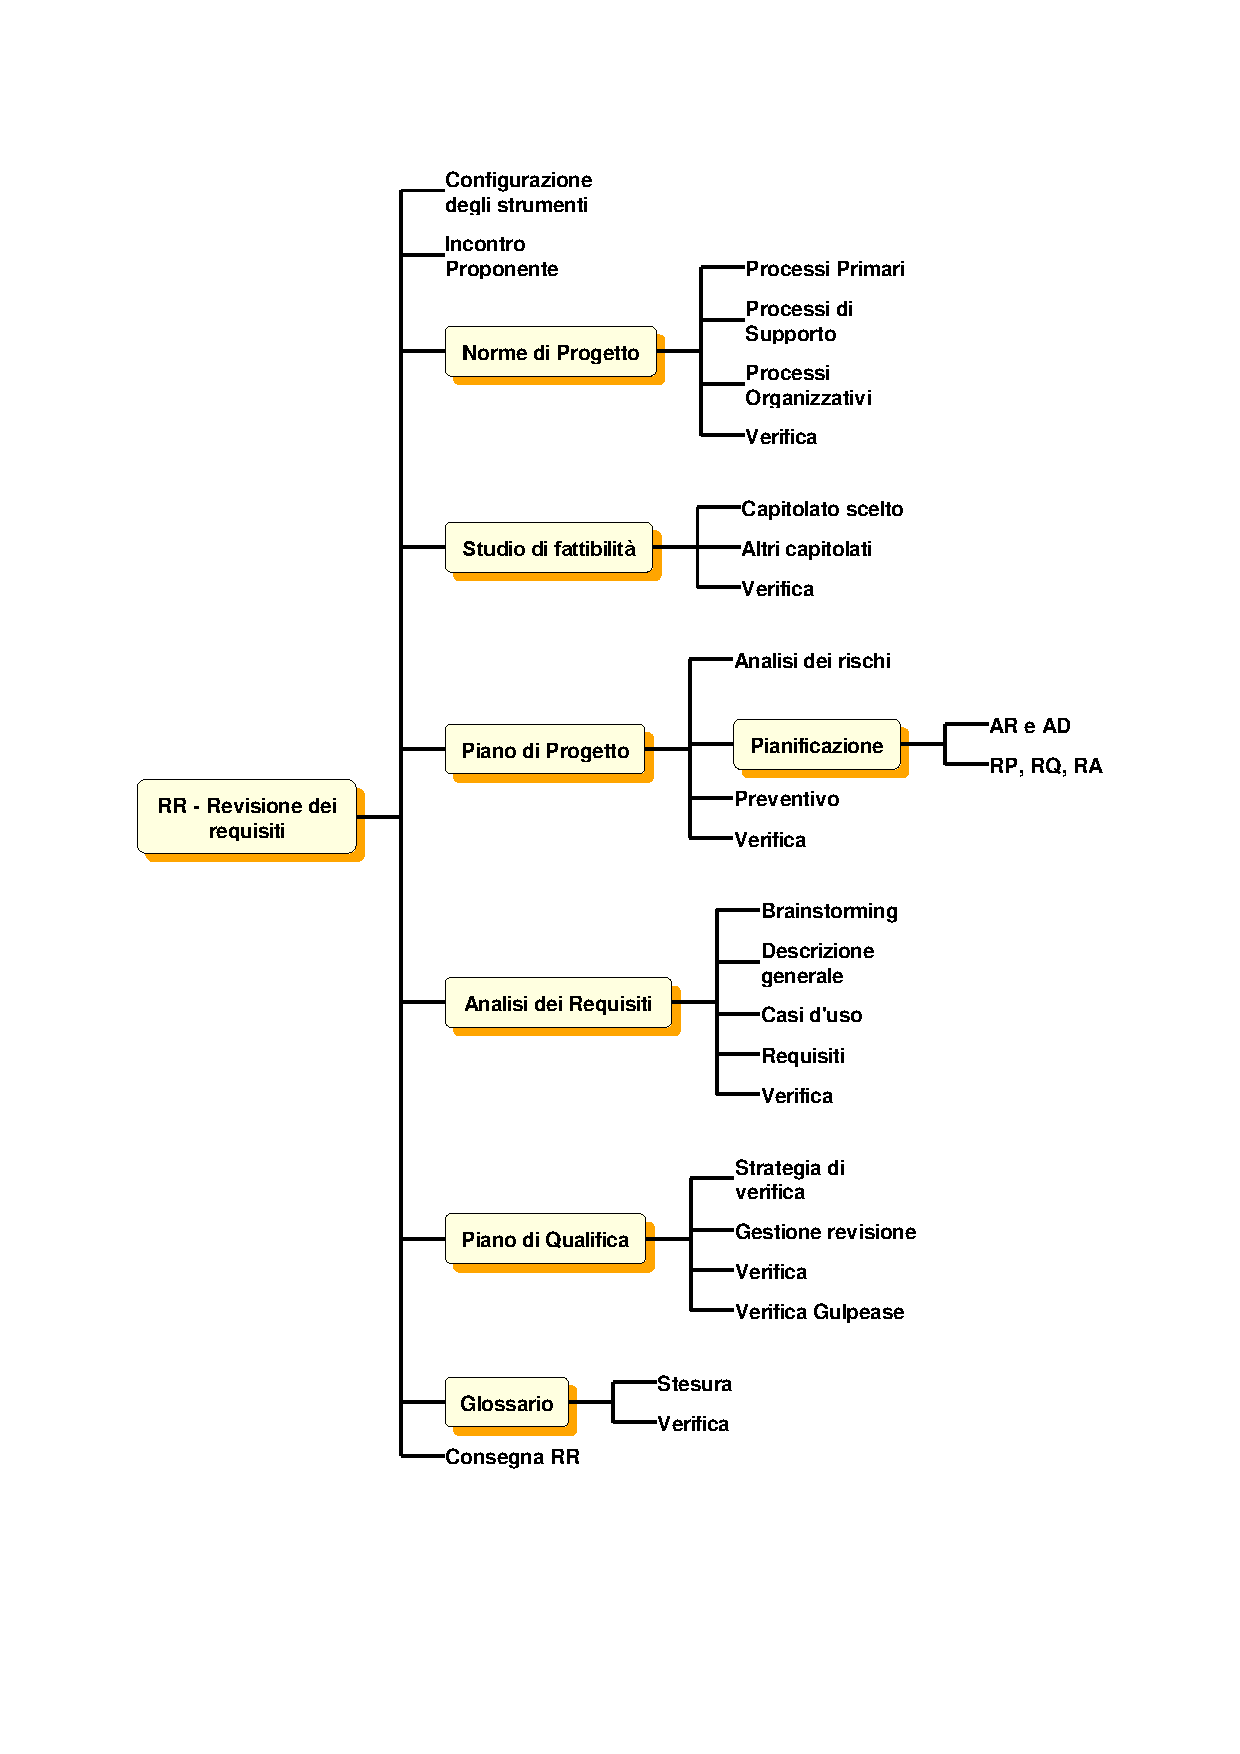
\includegraphics[width= 15cm]{immagini/ar_wbs.pdf}
	\caption{Diagramma WBS - Analisi dei Requisiti}
\end{figure}

\subsubsection{Diagramma di Gantt}
\begin{figure}[H]
	\centering
	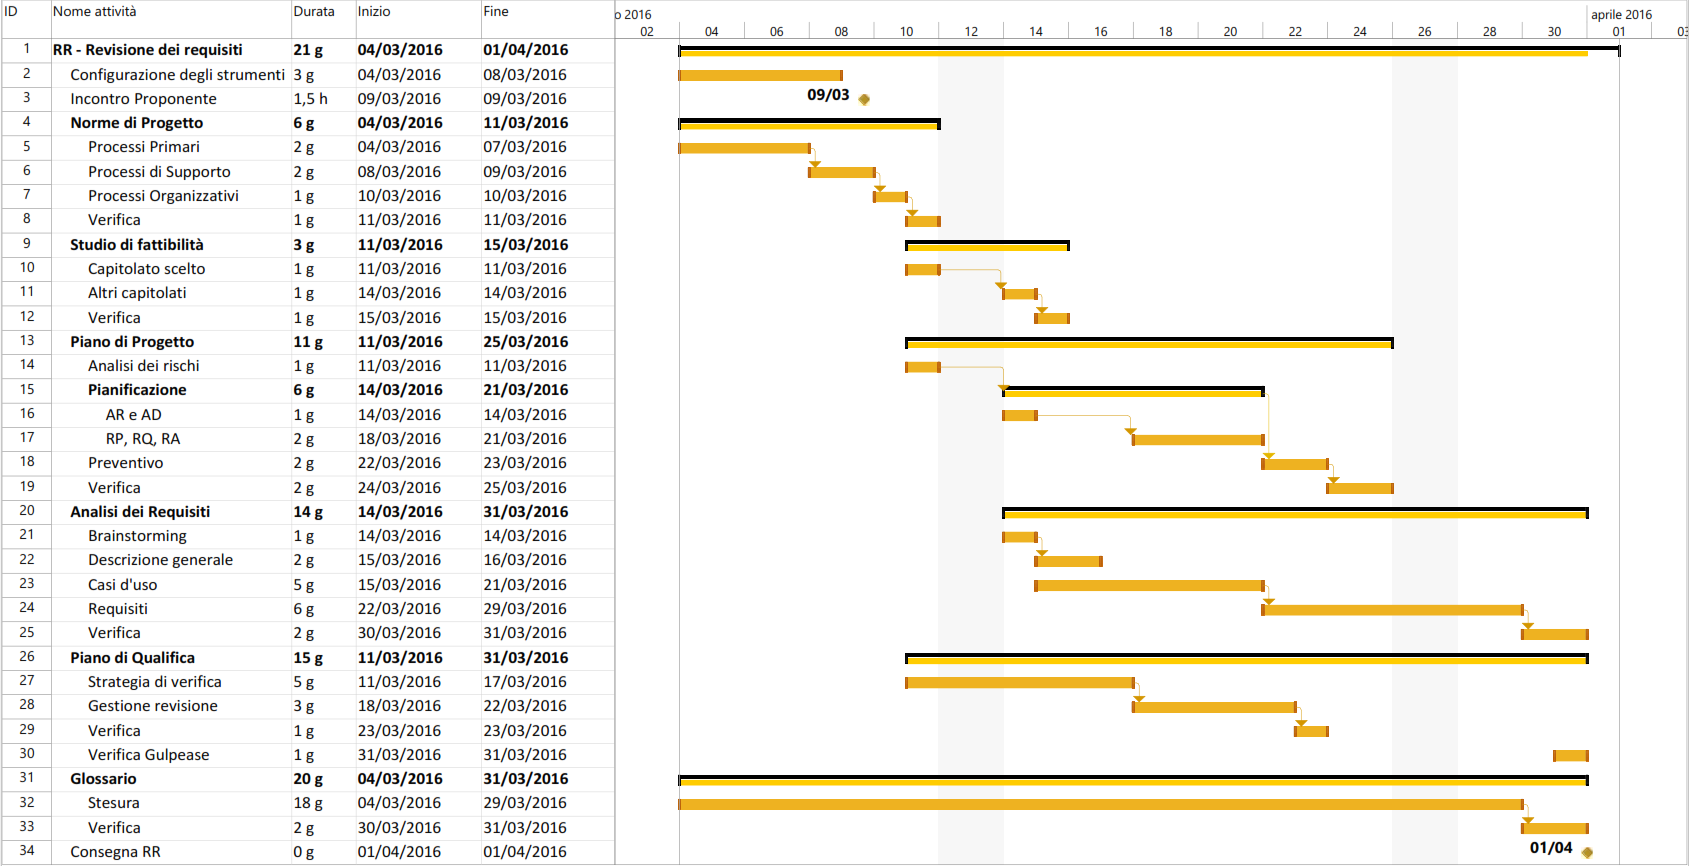
\includegraphics[width= 15cm]{immagini/ar_gantt.png}
	\caption{Diagramma di Gantt - Analisi dei Requisiti}
\end{figure}
\newpage

\subsection{Analisi di Dettaglio}
\textbf{Periodo:} 01/04/2016 - 18/04/2016\\
Questa attività ha termine con la presentazione pubblica in data 18/04/2016 
dell'Analisi dei Requisiti\\\\
I ruoli attivi in questa fase sono:

\begin{itemize}
	\item Responsabile;
	\item Amministratore;
	\item Analista;
	\item Verificatore.
\end{itemize}
In questa fase il gruppo consolida i requisiti precedentemente individuati e si 
prepara a presentare al committente i documenti sviluppati nella fase 
precedente, con l'ausilio di una presentazione PowerPoint\G.

\subsubsection{Diagramma WBS}
\begin{figure}[H]
	\centering
	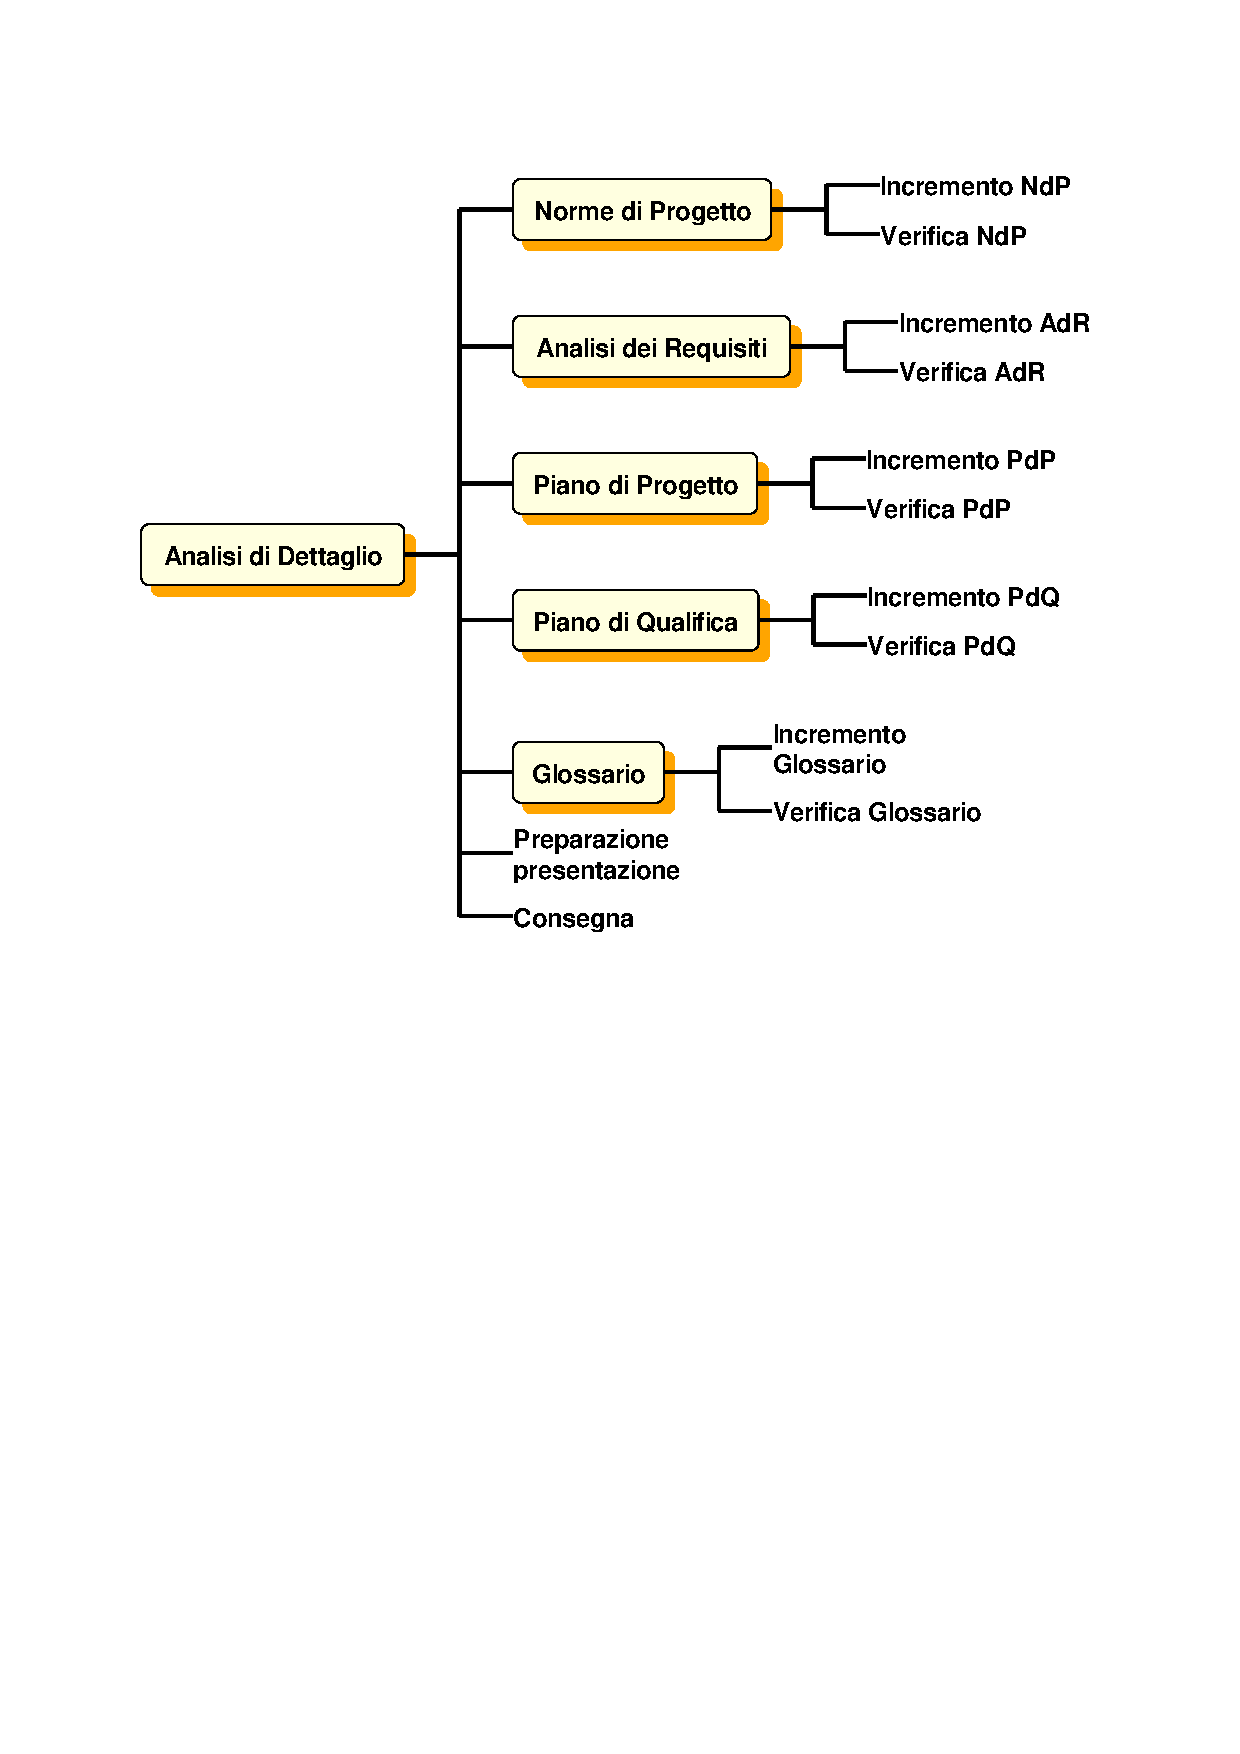
\includegraphics[width= 15cm]{immagini/ad_wbs.pdf}
	\caption{Diagramma WBS - Analisi di Dettaglio}
\end{figure}

\subsubsection{Diagramma di Gantt}
\begin{figure}[H]
	\centering
	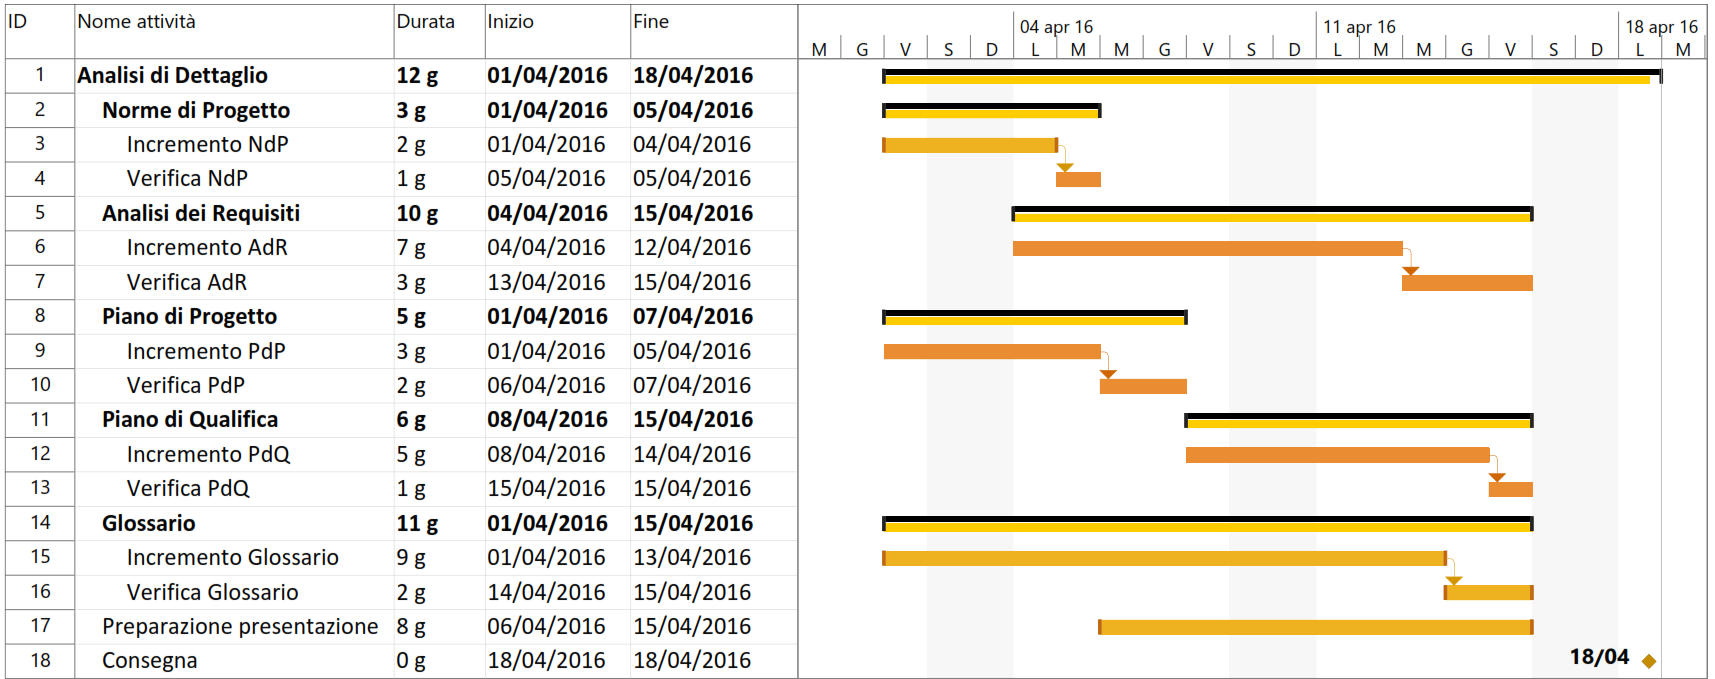
\includegraphics[width= 16cm]{immagini/ad_gantt.png}
	\caption{Diagramma di Gantt - Analisi di Dettaglio}
\end{figure}
\newpage

\subsection{Progettazione Architetturale}
\textbf{Periodo:} 19/04/2016 - 23/05/2016\\
Questa fase inizia il giorno 19/04/2016 e termina il 23/05/2016, giorno della 
Revisione di Progettazione. \\\\
I ruoli attivi in questa fase sono:

\begin{itemize}
	\item Responsabile;
	\item Amministratore;
	\item Analista;
	\item Progettista;
	\item Verificatore.
\end{itemize}
Il lavoro svolto dal gruppo in questa fase si divide in:
\begin{itemize}
	\item \textbf{Incremento}: tutti i documenti prodotti dall'Analisi dei 
	Requisiti verranno incrementati e corretti sulla base di segnalazioni 
	presentate dopo la prima consegna;
	\item \textbf{Specifica Tecnica}: compito dei progettisti è redigere il 
	documento di \textit{Specifica Tecnica v1.0.0}.
\end{itemize}

\subsubsection{Diagramma WBS}
\begin{figure}[H]
	\centering
	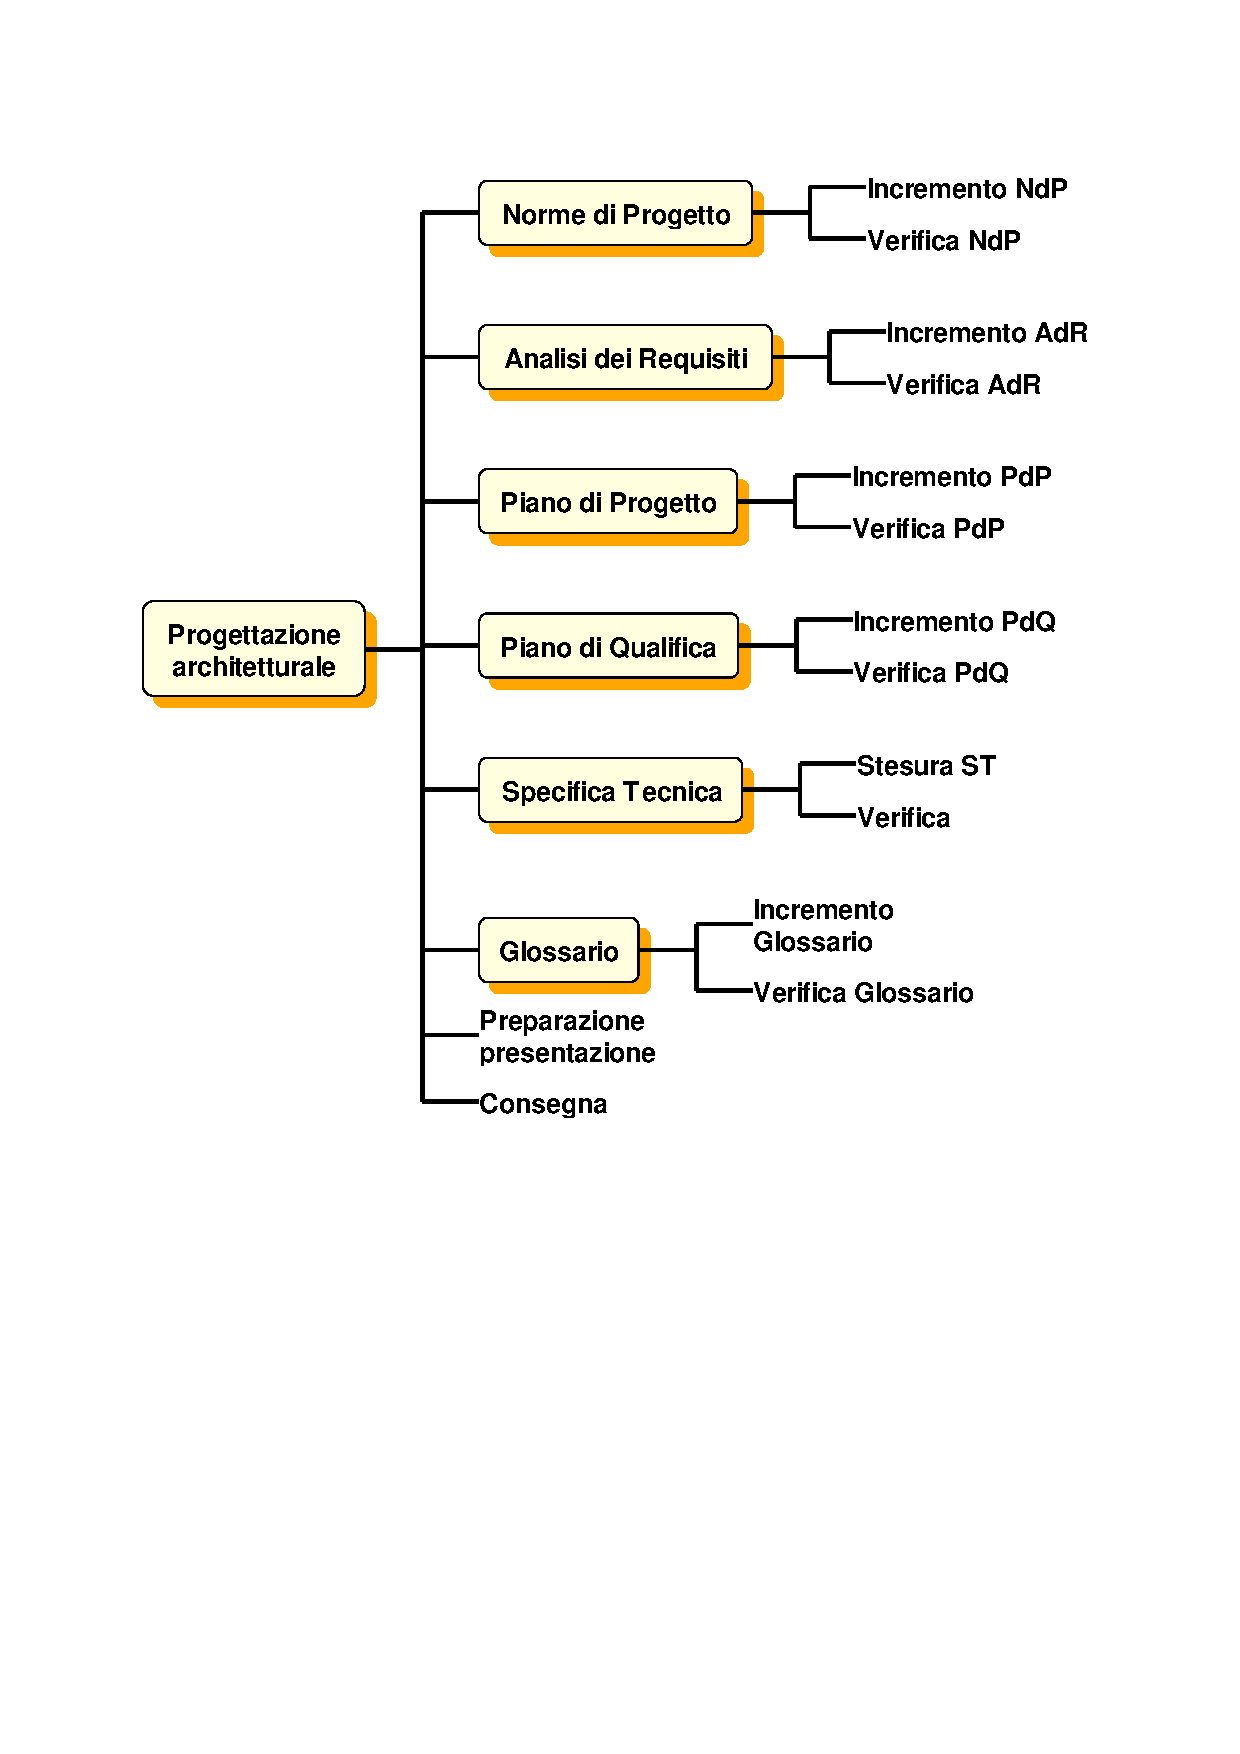
\includegraphics[width= 15cm]{immagini/pa_wbs.pdf}
	\caption{Diagramma WBS - Progettazione Architetturale}
\end{figure}

\subsubsection{Diagramma di Gantt}
\begin{figure}[H]
	\centering
	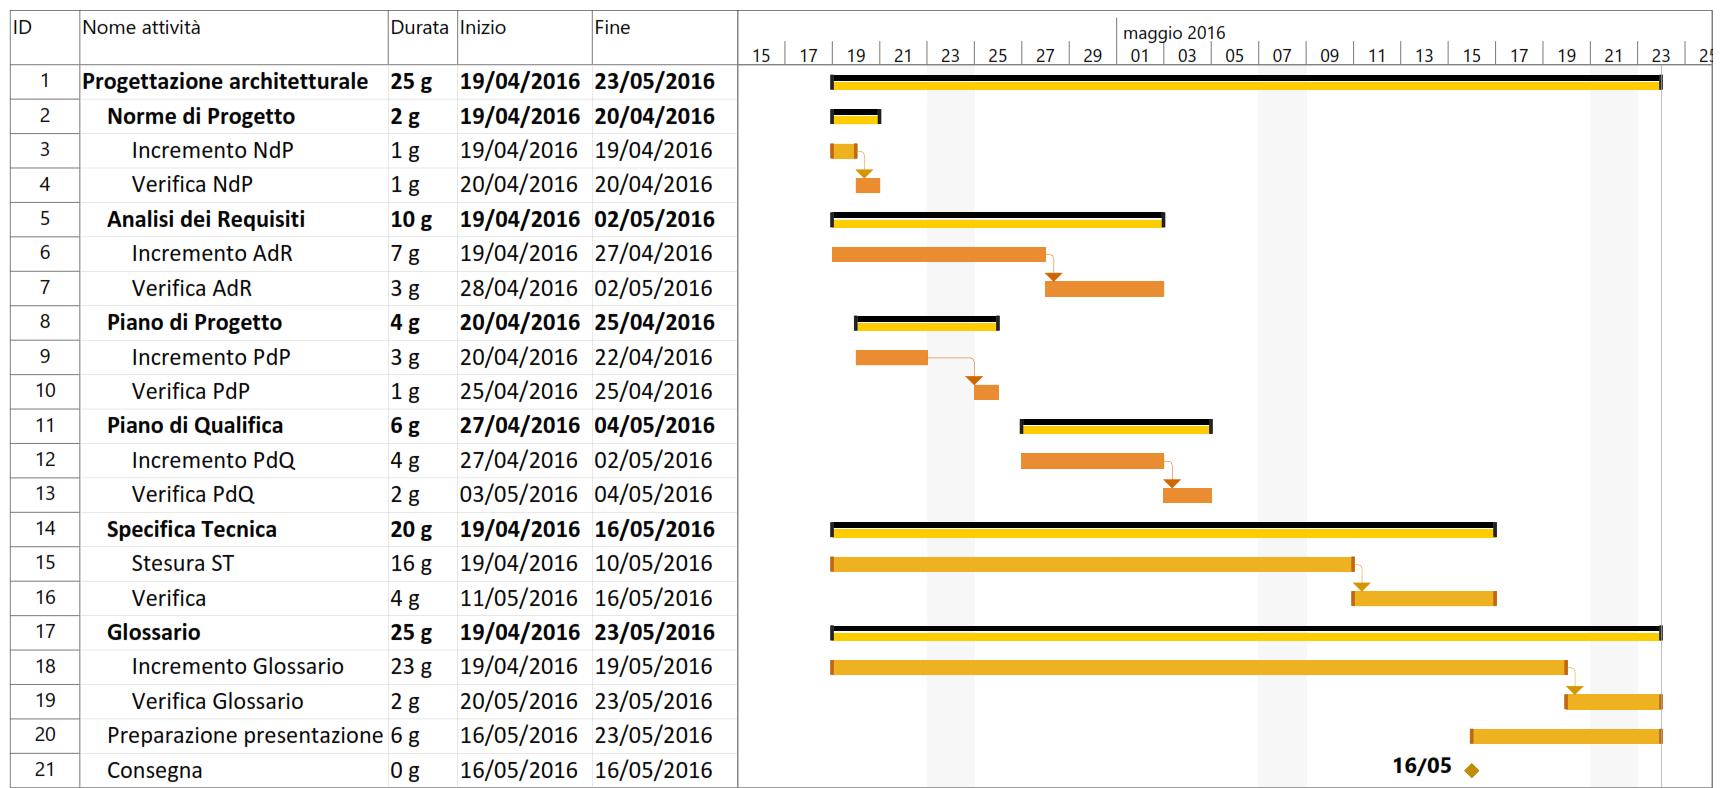
\includegraphics[width= 16cm]{immagini/pa_gantt.png}
	\caption{Diagramma di Gantt - Progettazione Architetturale}
\end{figure}
\newpage


\subsection{Progettazione di Dettaglio e Codifica}
\textbf{Periodo:} 24/05/2016 - 17/06/2016\\
Questa fase inizia il giorno 25/05/2016 e termina il 17/06/2016, giorno della 
Revisione di Qualifica. \\\\
I ruoli attivi in questa fase sono:

\begin{itemize}
	\item Responsabile;
	\item Amministratore;
	\item Analista;
	\item Progettista;
	\item Programmatore;
	\item Verificatore.
\end{itemize}
Il lavoro svolto dal gruppo in questa fase si divide in:
\begin{itemize}
	\item \textbf{Incremento}: tutti i documenti prodotti durante la fase di 
	Progettazione Architetturale vanno aggiornati;
	\item \textbf{Definizione di Prodotto}: il documento \textit{Specifica 
	Tecnica v1.0.0} descrive il modo in cui le varie componenti 
	del prodotto interagiscono fra loro. In esso vengono riportate le loro relazioni;
	\item \textbf{Codifica}: compito dei programmatori è sviluppare codice nel 
	linguaggio di programmazione stabilito;
	\item \textbf{Manuale Utente}: parallelamente allo sviluppo del codice si 
	provvede alla stesura del \textit{Manuale Utente v1.0.0}, necessario per guidare 
	l'utente verso un corretto utilizzo del \textit{software}.
\end{itemize}

\subsubsection{Diagramma WBS}
\begin{figure}[H]
	\centering
	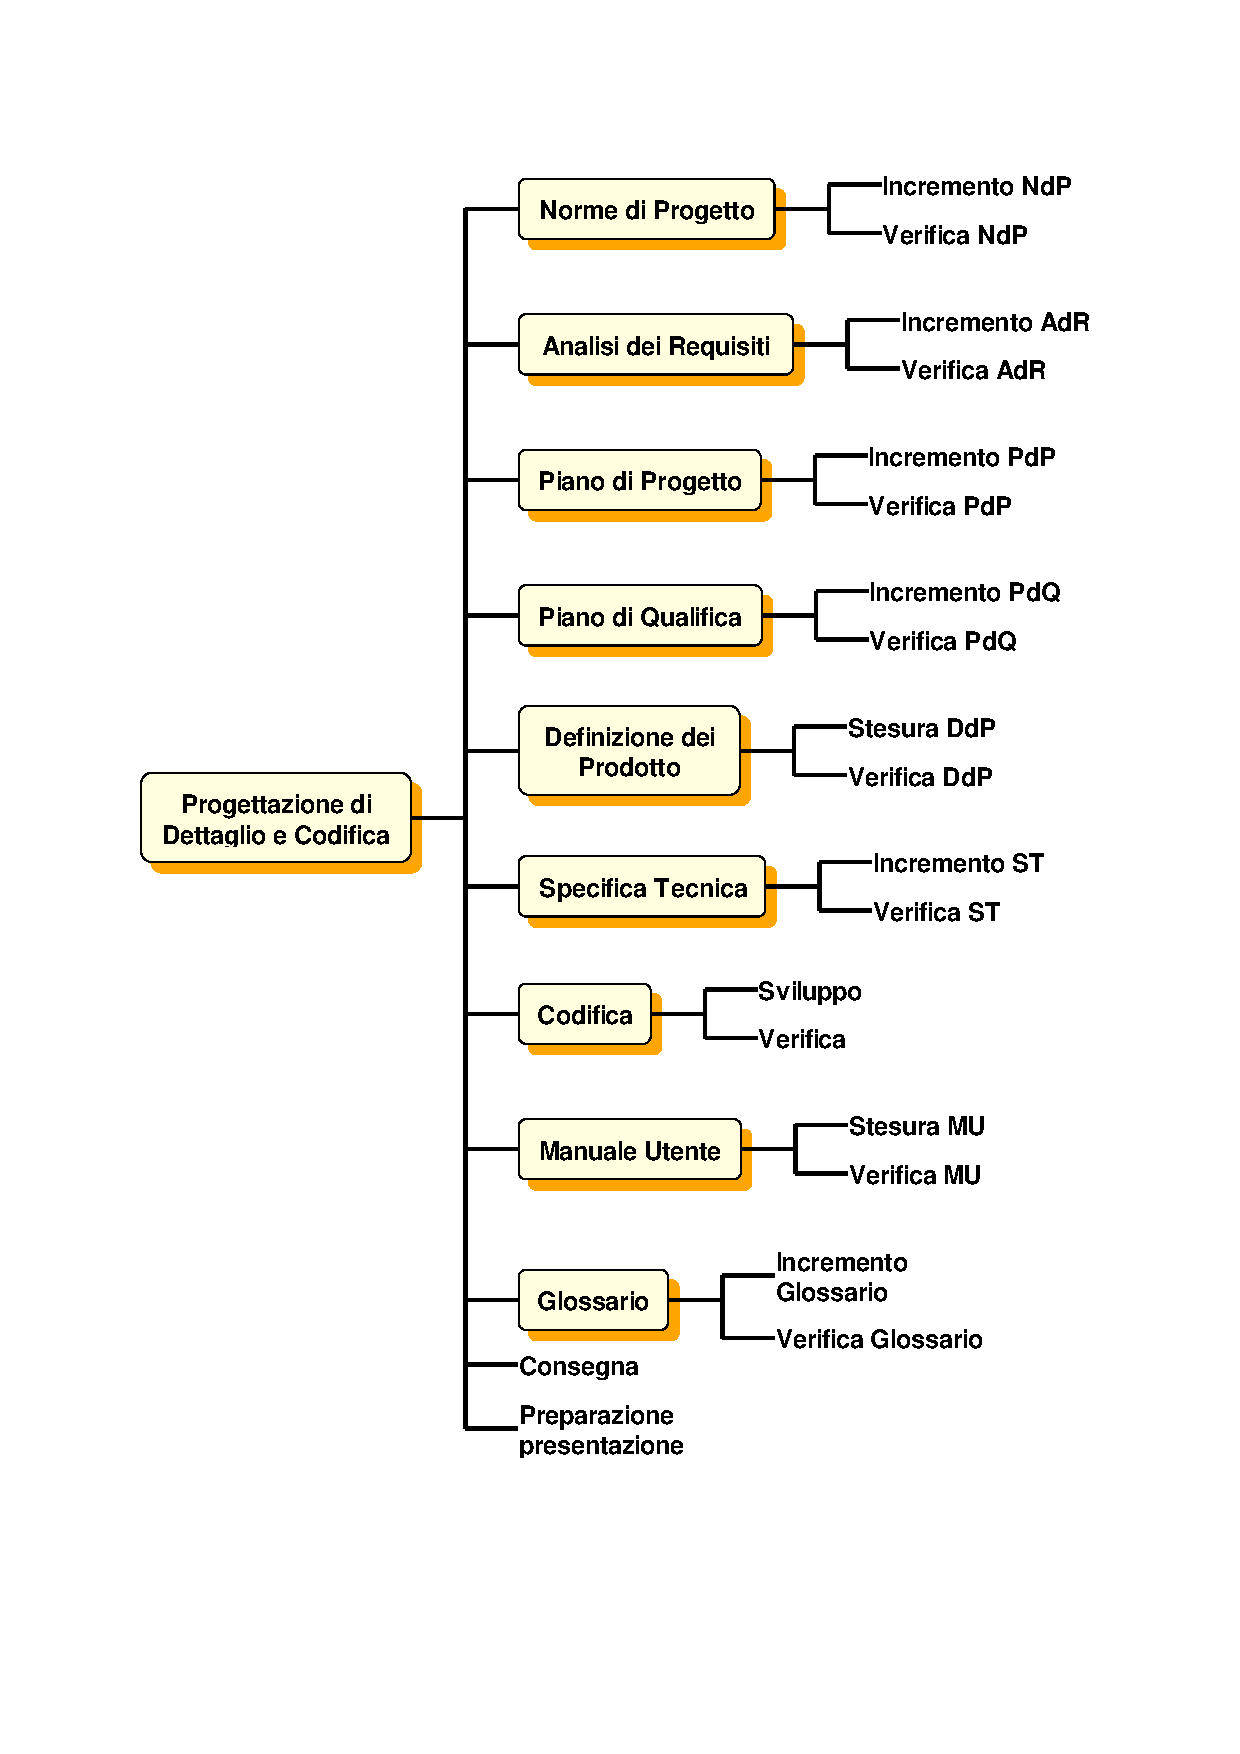
\includegraphics[width= 15cm]{immagini/pdc_wbs.pdf}
	\caption{Diagramma WBS - Progettazione di Dettaglio e Codifica}
\end{figure}

\subsubsection{Diagramma di Gantt}
\begin{figure}[H]
	\centering
	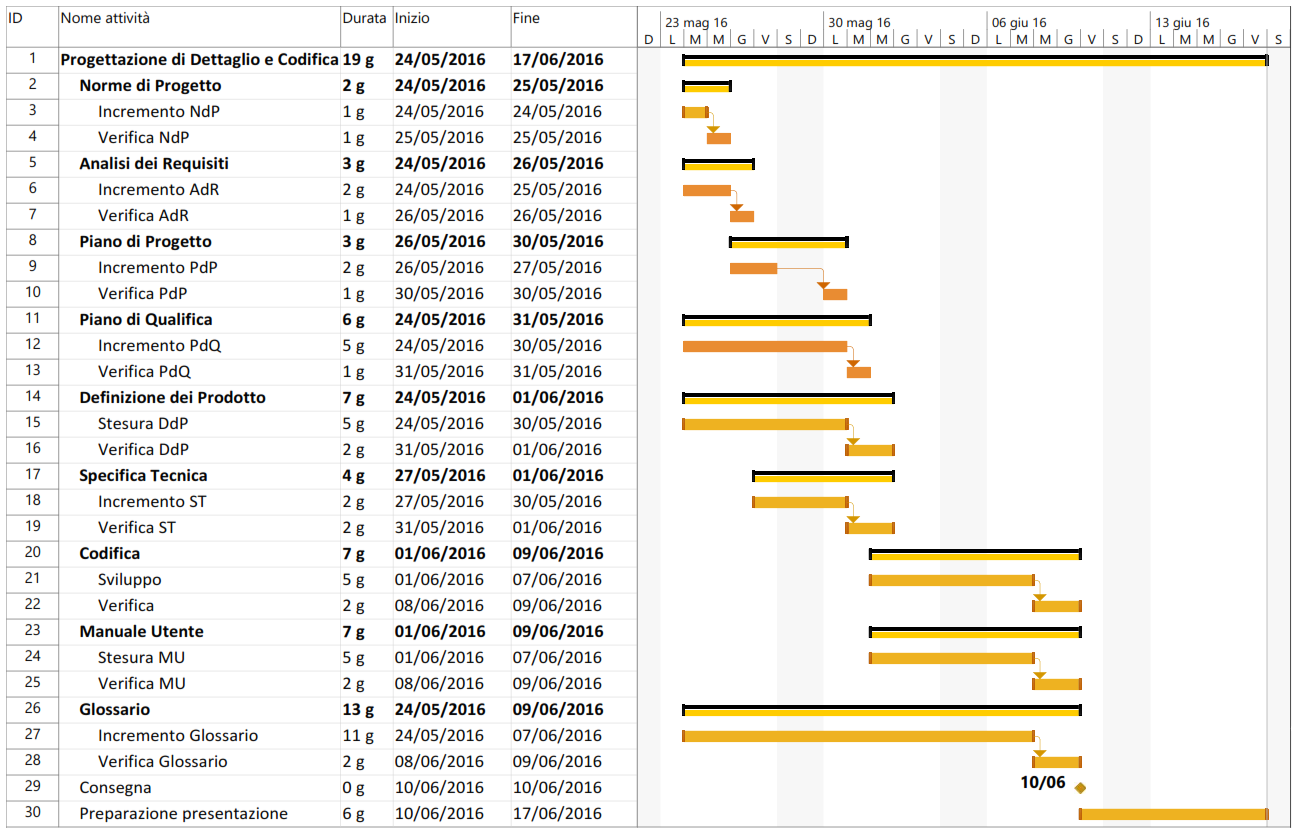
\includegraphics[width= 16cm]{immagini/pdc_gantt.png}
	\caption{Diagramma di Gantt - Progettazione di Dettaglio e Codifica}
\end{figure}
\newpage

\subsection{Validazione}
\textbf{Periodo:} 18/06/2016 - 11/07/2016\\
Questa fase inizia il giorno 18/06/2016 e termina il 17/06/2016, giorno della 
Revisione di Accettazione. \\\\
I ruoli attivi in questa fase sono:

\begin{itemize}
	\item Responsabile;
	\item Amministratore;
	\item Progettista;
	\item Programmatore;
	\item Verificatore.
\end{itemize}
Il lavoro svolto dal gruppo in questa fase si divide in:
\begin{itemize}
	\item \textbf{Incremento}: tutti i documenti prodotti durante la fase di 
	Progettazione di Dettaglio e Codifica vanno aggiornati;
	\item \textbf{Collaudo}: viene svolta un'accurata fase di \textit{testing} 
	per provare che tutti i requisiti specificati nell'\textit{Analisi dei 
	Requisiti v1.0.0} vengono soddisfatti.
\end{itemize}

\subsubsection{Diagramma WBS}
\begin{figure}[H]
	\centering
	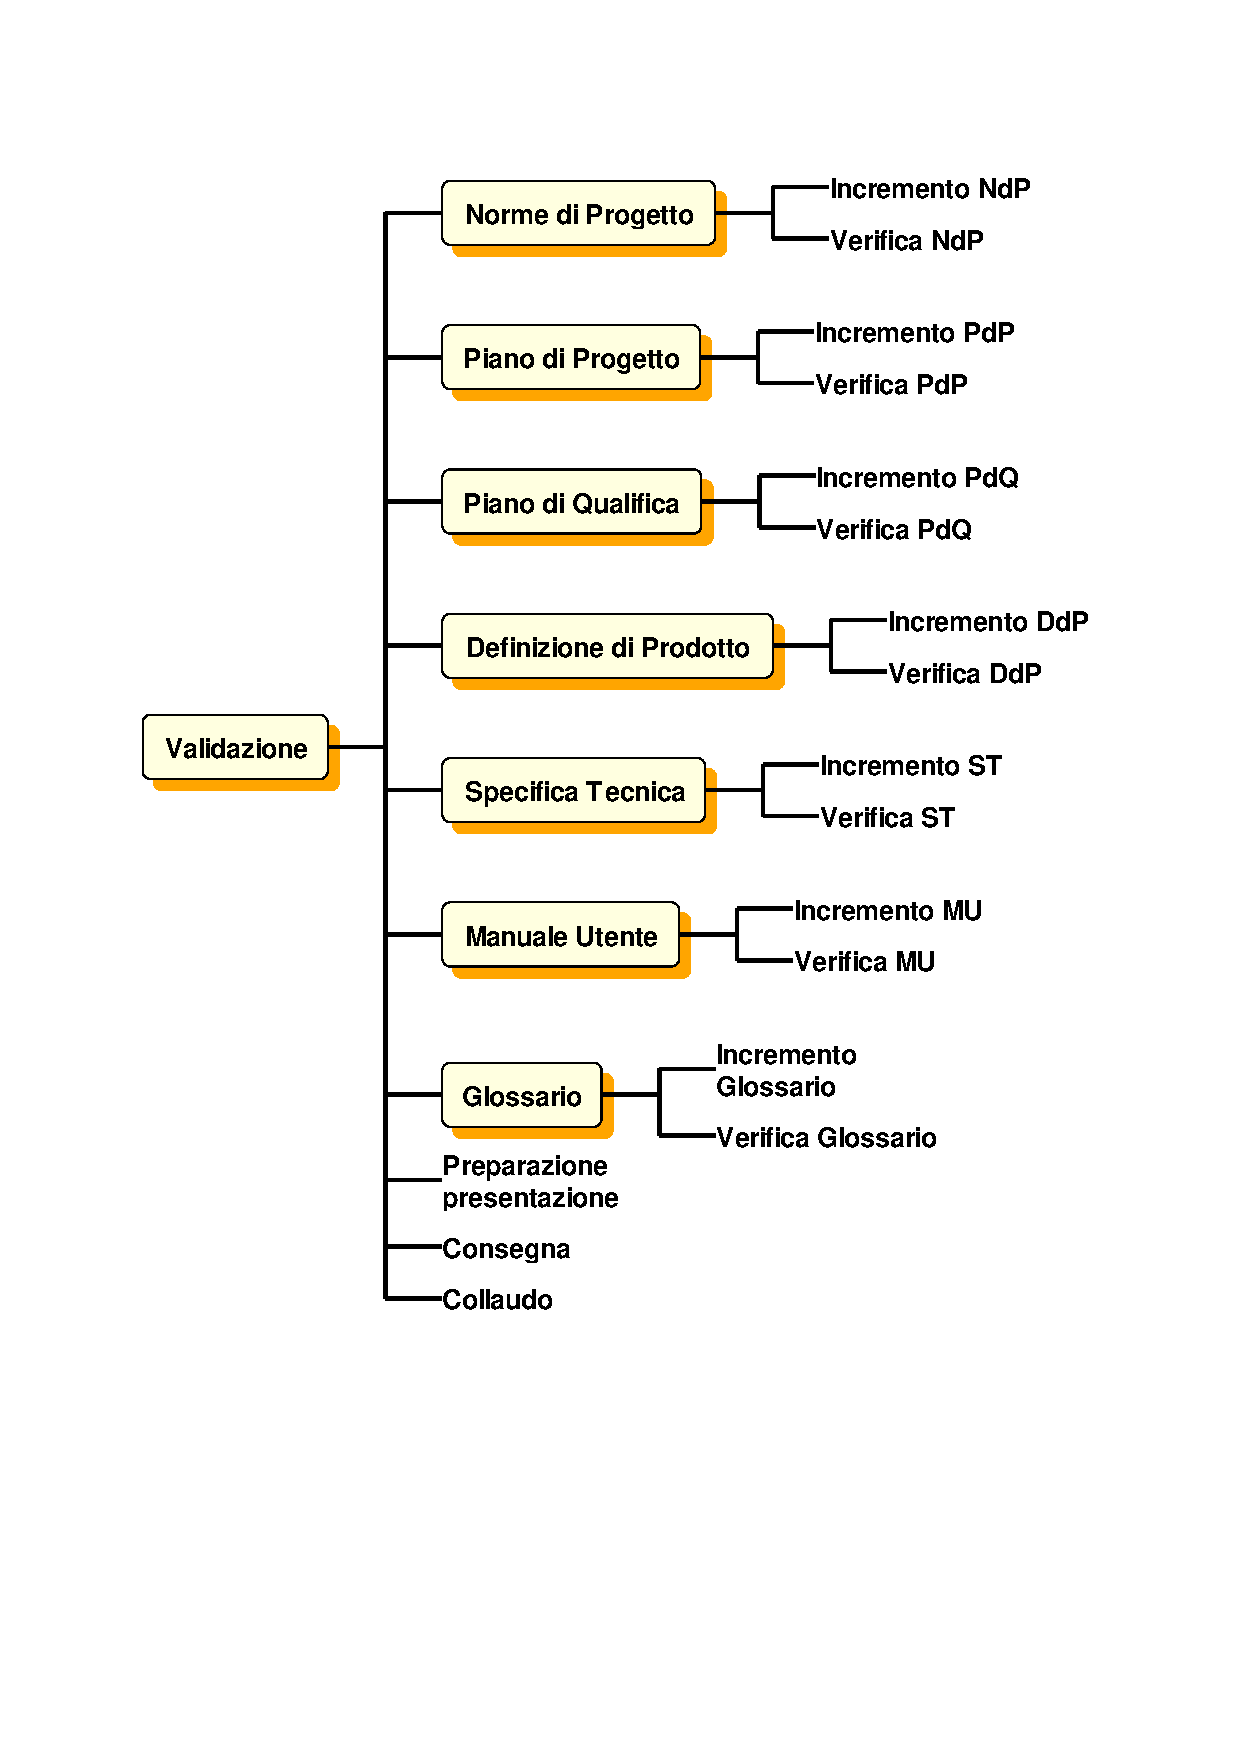
\includegraphics[width= 15cm]{immagini/va_wbs.pdf}
	\caption{Diagramma WBS - Validazione}
\end{figure}

\subsubsection{Diagramma di Gantt}
\begin{figure}[H]
	\centering
	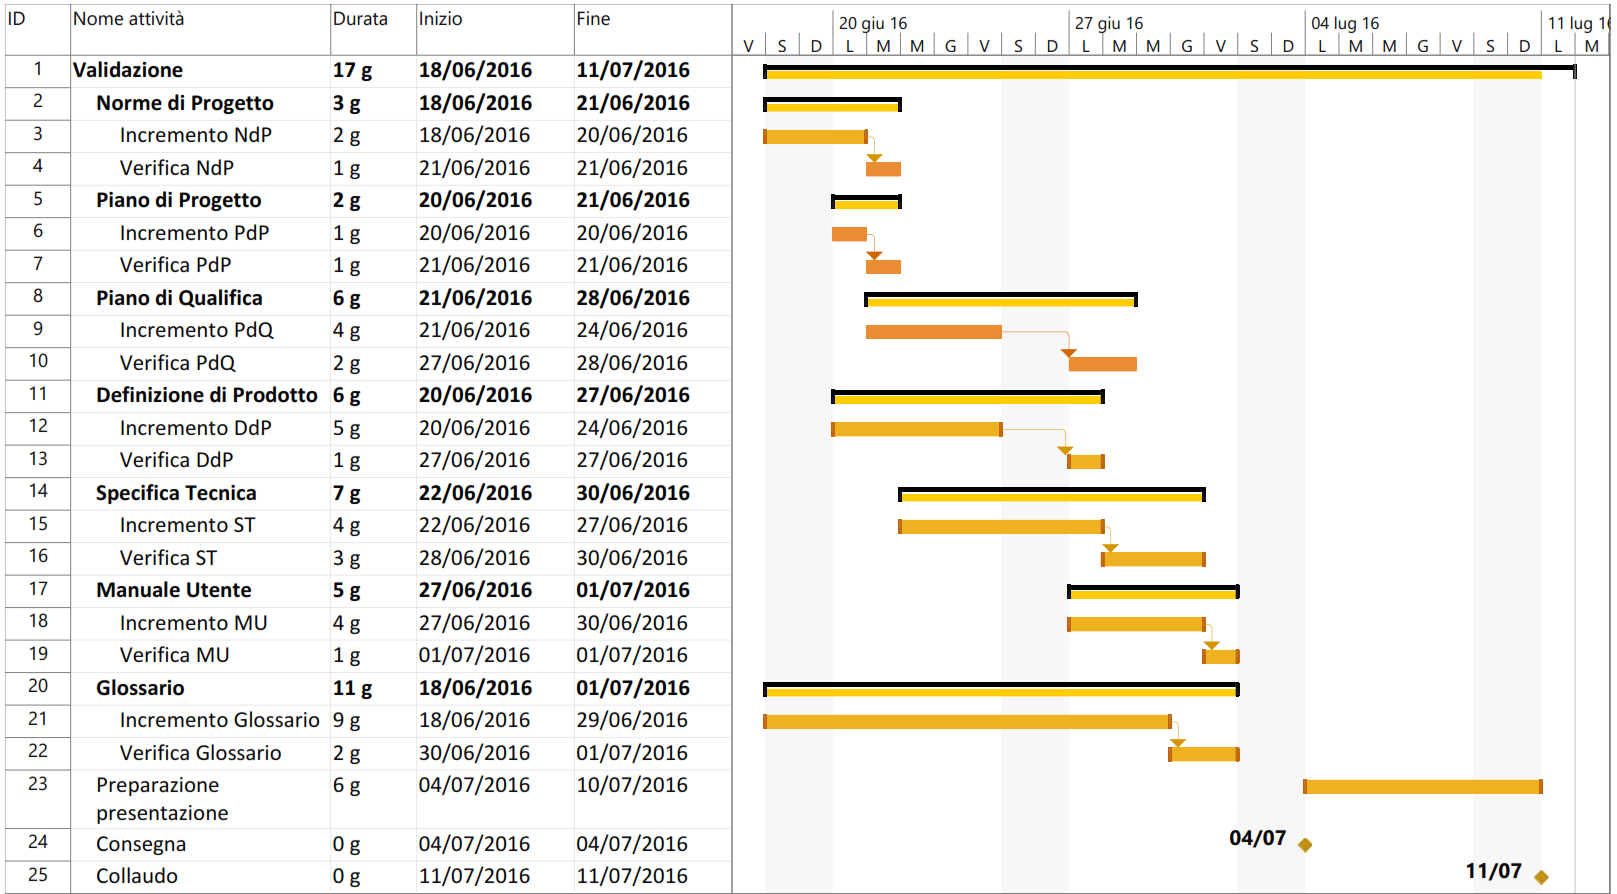
\includegraphics[width= 16cm]{immagini/va_gantt.png}
	\caption{Diagramma di Gantt - Validazione}
\end{figure}
\newpage